Sposób łączenia układu procesorów w sieć nazywamy topologią sieci. Topologię sieci można przedstawić jako graf \(G=(N,E)\), gdzie każdy węzeł \(i\in N\) oznacza procesor, a każda krawędź \((i, j) \in E\) – dwukierunkową komunikację między procesorami \(i\) i \(j\). Przyjmujemy, że każdy procesor ma swoją lokalną pamięć i nie ma żadnej pamięci współdzielonej przez procesory (rys. \ref{fig:model_net}). Tak jak w przypadku modelu z pamięcią wspólną, operacje w sieci mogą być synchroniczne lub asynchroniczne.\\

\begin{figure}[b]
\centering
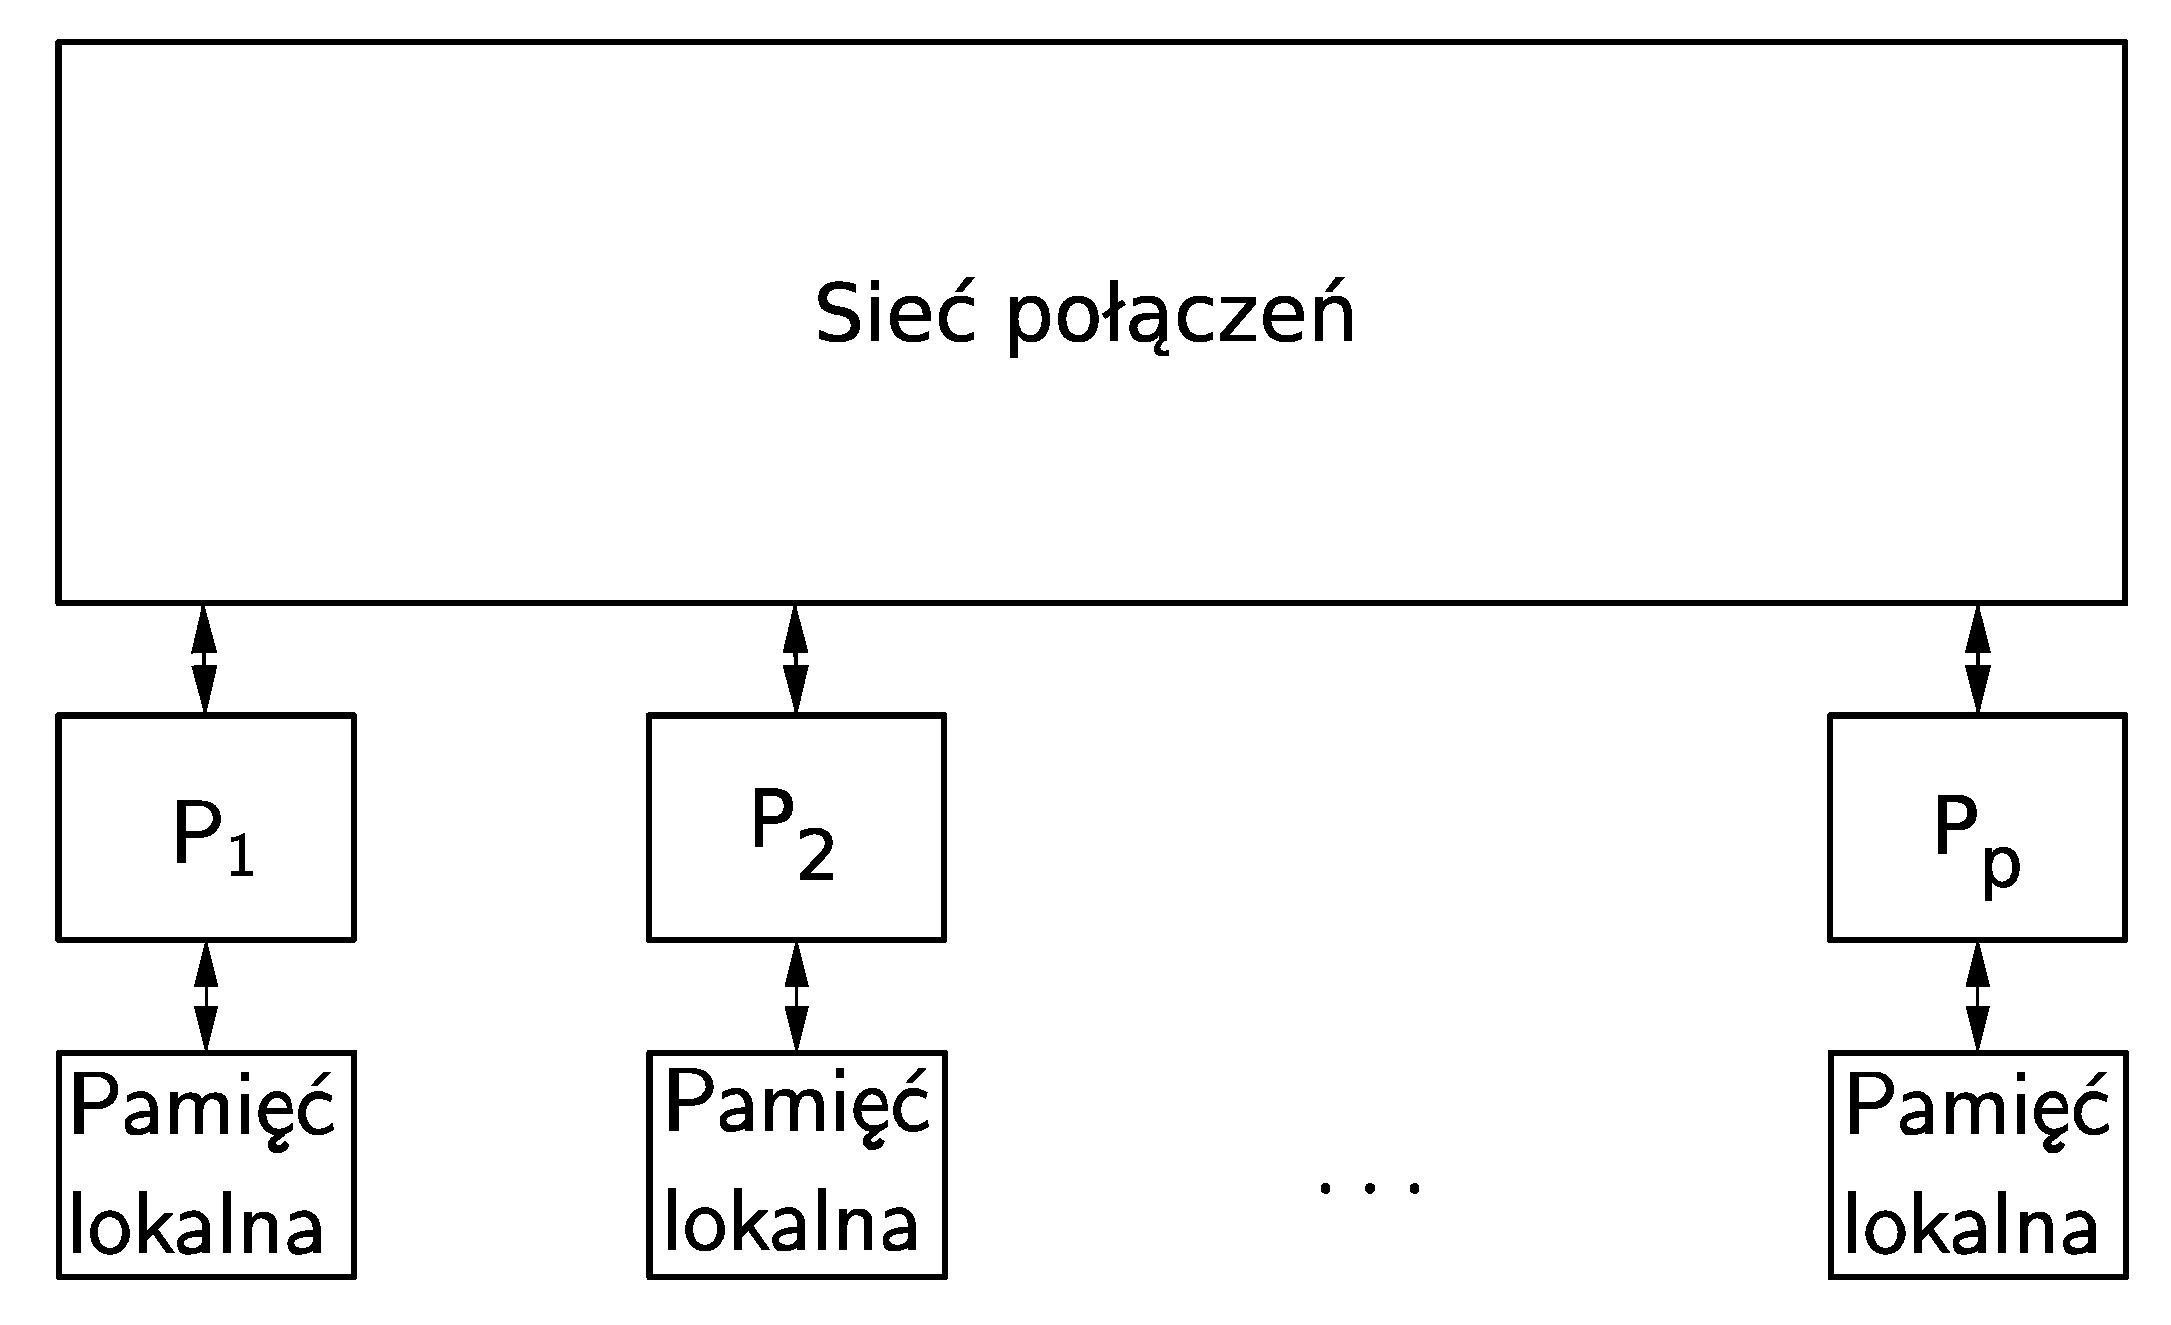
\includegraphics[width=22em]{images/Rys_net.eps}
\caption{Model wspólnej pamięci}
\label{fig:model_net}
\end{figure}

W opisie algorytmów dla modelu sieciowego potrzebujemy zdefiniować dwie instrukcje do opisania komunikacji między procesorami.
\begin{enumerate}
 \item send\((X,i)\)
 \item receive\((X,j)\)
\end{enumerate}

Procesor \(P\) wykonujący instrukcję \textbf{send} wysyła kopię \(X\) do procesora \(P_i\), następnie natychmiast przechodzi do wykonywania kolejnej instrukcji.\\
Procesor \(P\) wykonujący instrukcję \textbf{receive} zatrzymuje wykonanie programu aż do chwili, gdy otrzyma dane z procesora \(P_j\), a następnie przechowuje dane w \(Y\) i kontynuuje wykonanie programu.\\


Procesory pracujące w sieci asynchronicznej zarządzają swoimi zadaniami przez wymianę komunikatów. Schemat taki nazywamy modelem wymiany komunikatów. Procesory te niekoniecznie muszą być ze sobą sąsiadujące. 

%\begin{definicja}[Routing]
%Proces dostarczania każdego komunikatu od źródła do przeznaczenia nazywmy routingiem.
%\end{definicja}

Charakteryzuje ją kilka parametrów:

\begin{enumerate}
 \item średnica – maksymalna odległość (krawędziowa) między dowolną parą węzłów; im miejsza, tym lepiej.
 \item maksymalny stopień wierzchołka – maksymalna liczba łączy do dane procesora
 \item szerokość połowienia sieci – minimalna liczba krawędzi, które muszą zostać usunięty, aby podzielić ją na dwie równe podsieci
 \item spójność krawędziowa – minimalna liczba krawędzi, które muszą ulec awarii, aby sieć stała się niespójna
 \item koszt sieci – koszt wykonania, zarządzania i utrzymania połączeń między procesorami; w najprostrzym przypadku mierzony liczbą krawędzi
\end{enumerate}



\begin{przyklad}[Sieć liniowa]
Model składa się z \(p\) procesorów \(P_1, P_2, \dots, P_p\) połączonych ze sobą w ciąg, tzn. procesor \(P_i\) połączony jest z procesorem \(P_{i-1}\) i \(P_{i+1}\), o ile takie istnieją. Średnica takiej sieci wynosi \(p-1\), jej maksymalny stopień wynosi \(2\).\\
\end{przyklad}

\begin{przyklad}[Torus]
Siecią w topologii torusa nazywamy sieć liniowa z połączonymi końcami.
\end{przyklad}

\begin{przyklad}{Sieć dwuwymiarowa}
Dwuwymiarowa sieć jest dwuwymiarową wersją sieci liniowej. Składa się ona z \(p=m^2\) procesorów ułożonych w siatkę \(m\times m\) taką, że procesor \(P_{i,j}\) jest połączony z procesorem \(P_{i\pm 1, j}\) i \(P_{i, j\pm 1}\).\\
Średnica takiej sieci złożonej z \(p=m^2\) procesorów wynos \(\sqrt{p}\) a jej maksymalny stopień \(4\)
\end{przyklad}

\begin{definicja}{Kostka Boola}\\
Niech \(i_{d-1}i_{d-2}\dots i_{0}\), gdzie \(0\leq i \leq p-1\) będzie binarną reprezentacją \(i\). Wówczas procesor \({i}\) jest połaczony z procesorem \(P_{i^(j)}\), gdzie \(i^{(j)}=i_{d-1}\dots \overline{i_j} \dots i_0\) i \(\overline{i_j} = 1 - i_j\). Innymi słowy, dwa procesory są ze sobą połączone wtedy i tylko wtedy, gdy ich wskaźniki różnią się tylko jednym bitem.\\
\end{definicja}

\begin{przyklad}{Sieć hipersześcienna}
Sieć w topologii hipersześcianu skłąda się z \(p=2^d\) procesorów połączonych w d-wymiarową kostkę Boola.\\

Hipersześcian ma strukurę rekursywną. Kostkę \(d\)-wymiarową możemy rozszerzyć do \(d+1\) wymiarów przez połączenie poszczególnych procesorów do \(d\)-wymiarowych kostek.\\

Średnica d-wymiarowego hipersześcianu wynosi \(d=\log{p}\). Jest tak ponieważ odległośc w grafie między dwoma procesorami \(P_i\) i \(P_j\) jest równa liczbie pozycji bitów, którymi wskaźniki \(i\) i \(j\) różnią się między sobą. Stąd jest ona mniejsza lub równa \(d\), a ponadto odległość między \(P_0\) a \(P_{2^d-1}\) wynosi d. Każdy węzeł jest stopnia \(d=\log{p}\).
\end{przyklad}	
\begin{figure}[h]
\centering
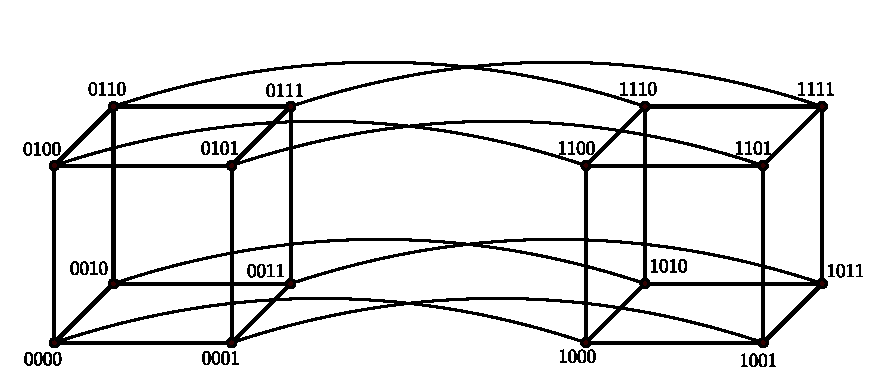
\includegraphics[width=32em]{images/systolic.eps}
\caption{Sieć w topologii hipersześcianu}
\label{fig:systolic}
\end{figure}
